\section{RHUL New Edwards Depositions\label{sec:edwards500}}
\newcommand{\imedwardsFiveHundred}{\hyperref[sec:edwards500]{\quote{\textbf{\underline{Edwards
          500}}}}}

Machine is located  in clean room, used  for depositing \textbf{gold,
  nickel, titanium  aluminium.} \red{Very important to  get the valve
  system in the right order.}
\subsection{Switching machine on}
The machine is initially  in the off state. First we  need to get the
pumps of the machine up and running.
\begin{enumerate}
\item  On the  black `button  board' \cmd{turn  the dial  on the  top
    middle sector from 0 to 1} to turn the machine on.
\item  The   green  screen  directly   to  the  right   should  light
  up. \texttt{Select `MANUAL MODE'} out of the possible options.
\item     \texttt{Scroll    to     ``RELAY-INPUTS''    \ira     Press
    ``YES''}. \red{Check that everything is \quote{OFF}!}
\item \cmd{Go  to \quote{1 ROT  PUMP} option \ira  press \quote{ON}.}
  This turns on the rotary pump.
\item \cmd{Go to \quote{3 BACKING  V.} option \ira press \quote{ON}.}
  Now the turbo molecular pump is being pumped.
\item \cmd{Go  behind the machine,  and check  that the black  box is
    receiving power.} Red light below \quote{POWER IN} should be on.
\item Open  up the chamber directly  under the main chamber.   At the
  very back is  th turbo molecular pump switch -  \red{A red switch.}
  \cmd{Flick it \red{down}  to start the turbo molecular  pump. If it
    starts flashing red, turn it on and off again.}
\end{enumerate}

 \begin{figure}[htbp]
   \centering 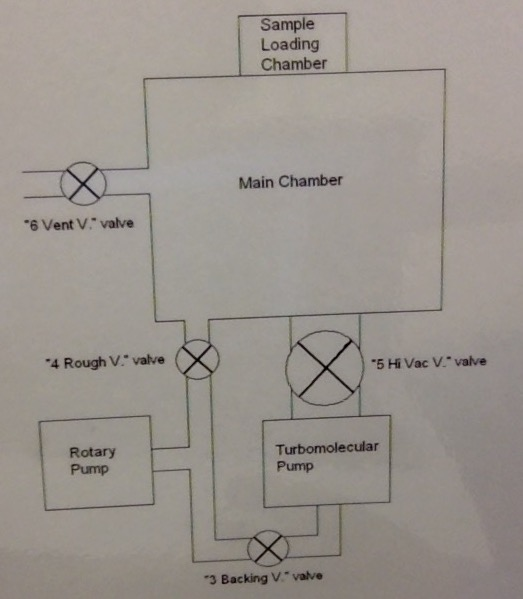
\includegraphics[height=10cm]{dia}
 \end{figure}
 \subsection{Loading}
 To load, we need to vent  the chamber and open the door.  \red{Prior
   to loading  double check  that \cmd{\quote{4 ROUGH  V.} \quote{5
       HIGH VAC V.}} are off!}
 \begin{enumerate}
 \item \cmd{Press \ino \ira \imonitor  \ira Go to \ipenning menu \ira
     Press \iyes to enter.}
 \item  \cmd{\iheadon will  be displayed  \ira Press  \iyes \ira  Now
     reads \iheadoff.}   We need to  turn off the sensitive  gauge to
   avoid damaging it.
 \item \cmd{Go  to ``6 VENT  V'' options \ira Will  read \quote{OFF}
     \ira Press \quote{YES} \ira Will go to \quote{ON}};
 \item \cmd{Press \ino  \ira Will read \imonitor \ira  Press \iyes to
         enter menu.} Chamber pressure displayed;
   \item When pressure gauge read $ 10^3 $MB, \cmd{Press \ino.}
         \item If too slow, open valve3 on top
 \item \cmd{Go to \irelayinputs \ira Press \iyes};
 \item \cmd{Go to \ivent option \ira Reads \ion \ira Press \iyes \ira
     Now reads  \ioff.} \red{THIS IS SO  WE DONT FORGET TO  CLOSE THE
     VALVE AFTERWARDS AND SCREW UP THE TURBO PUMP};
 \item Chamber can now be opened and loaded;
 \item Check  the material level  by \cmd{Go to TURRET  CONTROL PANEL
     \ira  Select material  \ira Press  the ``0/1  BUTTON'' \ira  The
     motor  switches on.\ira  Remember to  switch the  ``0/1 BUTTON''
     off.}
 \end{enumerate}

 \subsection{Pumping the main Chamber}
 Once the sample is loaded
 \begin{enumerate}
 \item \cmd{Go to \irelayinputs \ira Press \iyes.}
 \item \cmd{Go  to \ivent option  \ira Check  if reads \ioff  (If not
     press \iyes to set to to \ioff.)} This is to prevent the venting
   of the main chamber.
 \item \cmd{Go  to \ibacking option  \ira Press \iyes \ira  Now reads
     \ioff}. This is to isolate the turbo pump from the main chamber.
 \item  \cmd{Go to  \irough option  \ira Press  \iyes \ira  Now reads
     \ion.} This causes the rotary pump to pump the main chamber.
 \item  \cmd{Press \ino  Now reads  \imonitor \ira  Press \iyes  \ira
     Chamber pressure displayed. Wait until 0.5MB reached.}
 \item \cmd{Press \ino \ira Go to \irelayinputs \ira Press \iyes.}
 \item   \cmd{Go  to   \irough   \ira  Press   \iyes\ira  Now   reads
     \ioff. \red{Wait 10-15 seconds.}}  This prepares the rotary pump
   for helping the turbo one.
 \item \cmd{Go  to \ibacking option  \ira Press \iyes \ira  Now reads
     \ion.} We now pump the turbo pump with the normal one.
 \item \cmd{Go  to \ihighvac option  \ira Press \iyes \ira  Now reads
     \ion.} The turbo pump is now pumping the main chamber.
 \item \cmd{Press  \ino \ira  Go to \imonitor  \ira Press  \iyes \ira
     \red{Check pressure is decreasing.}}
 \item \cmd{Press \ino \ira Go to \ipenning menu \ira Press \iyes.}
 \item \cmd{Press \iyes  \ira Now reads \iheadon.} This  turns on the
   sensitive pressure meter.  If it  doesn't turn on, repeat until it
   does.
 \item \cmd{Press  \ino \ira  Go to \imonitor  \ira Press  \iyes \ira
     \red{Leave to pump until $ 5*10^{-5} $MBar}.}
 \end{enumerate}


 \subsection{Crucible deposition}
 \begin{enumerate}
 \item \textbf{TURRET CONTROL}  is where one selects  the material to
   deposition. \cmd{Turn the dial to  the desired position \ira Press
     the  ``0/1 Button''  to activate  the  motor and  make it  turn.
     Remember to turn it off  afterwards though.  \cmd{On}} means the
   motor it running, \cmd{o$ \backslash $l}  means it is not moving.  A yellow
   light indicates the turret position;
 \item \textbf{SWEEP CONTROL} is where  one adjusts the beam. The raw
   settings are
   \begin{itemize}
   \item X = z waveform, \red{15 frequency}, middle amplitude;
   \item Y = sinusoid waveform, \red{8 frequency}, middle amplitude.
   \end{itemize}
 \item  \textbf{SOURCE CONTROL}  is where  one sets  the accelerating
   voltage and the current for crucibnle deposition.
 \item \red{\textbf{SOURCE SHUTTER} \ira \cmd{Press middle button} to
     set  it  into  remote  mode.  This  way  whenever  the  required
     thickness  is  reached (via  LabView  or  manual procedure)  the
     shutter will close automatically.}   \red{If you want to control
     the  shutter manually,  \cmd{Do  NOT press  the middle  button.}
     Instead be prepared  to \cmd{Press SS1 button}  (left hand side)
     to open and close to the shutter manually.}
 \item  Activate  the  \textbf{\quote{FTM7}}   where  one  sets  the
   deposition  parameters.   \cmd{Click  on \quote{DATA}  button  to
     change    between    the   menus.}     \red{Alternatively    run
     \quote{FTM7\_set\_parameters.vi}  from   LabView  to   set  the
     material and thickness! }
   \begin{itemize}
   \item \textbf{Rate} gives the current deposition rate;
   \item \textbf{Layer} is what material is being deposited. There is
     a  sheet  in the  lab  saying  what  layer corresponds  to  what
     material.   E.g. for  Au it  it layer  4.  \cmd{\red{Set  to the
         required material!}};
   \item \textbf{Density  and z-Value (acoutstic impedance)}  are set
     depending on the layer chosen.  They depend on the material used
     - \red{\cmd{set to the required material.}};
   \item \red{\textbf{Terminate}  is were we set  the thickness after
       which  to  close  the  shutter.   \cmd{\red{Set  the  required
           thickness.}};}
   \item  \textbf{Tooling} sets  the ratio  of the  distances of  the
     quartz   thickness   crystal   and    the   samples   from   the
     crucible. \red{Set to 1.0}
   \item \textbf{xTal} selects which of the 2 crystal we are going to
     use. \red{By default set to 1 - \textbf{the crystal in the right
         hand side of the chamber}}
   \item \textbf{Usage} indicates how much  the crystal has been used
     out of 100\%.
   \end{itemize}
 \end{enumerate}

 With this basic setup, one can proceed via two routes to perform the
 deposition.

 \subsubsection{Gun deposition (i.e. we do it manually)}
 \begin{enumerate}
 \item \cmd{Set the deposition parameters on \quote{FTM7}.}
 \item  \cmd{Go  to  \quote{SWEEP   CONTROL}  panel  turn  the  dial
     \red{0$ \rightarrow $ 1.}}
 \item   \cmd{Go  to   \quote{SOURCE  CONTROL}   panel  \ira   Press
     \quote{ON/OFF}.}
 \item  \cmd{Press \quote{GUN}  button to  allow local  control \ira
     Voltage should jump to \red{5kV}.}
 \item \cmd{Slowly ramp up the current 0mA\ira20mA\ira40mA\ira\red{No
       more  than 120mA!}   and monitor  the deposition  rate on  the
     \quote{FTM7} panel.}
 \item  When  a  steady  reading is  produced  (0.10nm/s)  \cmd{Press
     \quote{RUN} on  the \quote{FTM7}  panel to open  the shutter}.
   Deposition proceeds, and the shutter will close automatically once
   the \red{set thickness  is reached}. Shutter can be  out in manual
   mode  by  `unpressing'  the  \quote{REMOTE  SHUTTER}  button  and
   operating the \quote{SS1} button.
 \item  \red{Make   sure  that  there   are  no  explosions   in  the
     crucible. Lower current if required.}
 \item Once  done, shutter will  close. \cmd{Slowly ramp  the current
     down   to  0   \ira  Turn   off  \quote{GUN}   \ira  Turn   off
     \quote{SOURCE CONTROL} \ira Turn off \quote{SWEEP CONTROL}.}
 \end{enumerate}

   \subsubsection{Local/Remote deposition (usingLabView\label{sssec:depositLab})}
   LabView  is when  the deposition  is controlled  from the  LabView
   program.

   \begin{enumerate}
   \item \cmd{Log into \quote{Administrator} with empty password.}
   \item \cmd{Load \cmd{Evaporation Control Program.}}
   \item  \cmd{Choose  material  \ira choose  thickness  \ira  choose
       rate. Do not  worry about the turret option -  then turret you
       have  set  manually is  the  one  that  will  be used  in  the
       deposition.} \red{\cmd{Run program \ira  press start \ira wait
         until shutter lights turns on  and off \ira stop program} to
       set parameters on \quote{FTM7}.}
   \item  \cmd{Go   to  \quote{SOURCE  CONTROL}  panel   \ira  Press
       \quote{ON/OFF} \ira Voltage should jump to \red{5kV}.}
   \item \cmd{Press \quote{LOCAL/REMOTE} button  to allow LabView to
       control the current.}
   \item \cmd{RUN  the program.}  The  rate will be  reached (current
     10-100mA) \ira Shutter opened  \ira Set thickness deposited \ira
     Shutter  closed  \ira current  ramped  down.   \red{If an  error
       occurs, manually lower the  current by slowly lowering current
       value in \quote{Electron Gun.vi} to 0mA.}
   \item Turn off \quote{REMOVE/LOCAL}  \ira Turn off \quote{SOURCE
       CONTROL} \ira Turn off \quote{SWEEP CONTROL}.
   \end{enumerate}
   \subsection{Boat or spiral deposition}
   \red{There is no shutter for this  deposition! We do not touch the
     source control panel,  but use the one with HT,  LT and big 0-11
     dial}

   \begin{itemize}
   \item \cmd{Set the deposition parameters on \quote{FTM7}.}
   \item  \cmd{\red{\textbf{Ensure  that  the middle  source  shutter
           button  is  NOT  pressed}}   \ira  press  \quote{Run}  on
       \quote{FTM7}} to begin accumulation from 0;
   \item The front and back voltage supplies are chosen \cmd{using LT
       selectors \quote{front} and \quote{back} respectivily};
   \item \cmd{Choose \quote{LT} on the LT-O-HT dial} to activate the
     voltage supply;
   \item \cmd{\quote{Reset} and begin ramping up the current};
   \item \cmd{Once  \quote{FTM7} shows  the required  thickness \ira
       \red{press \quote{trip}} and turn the dial to LT-0-HT}
   \end{itemize}

 \subsection{Venting the main chamber}
 Once the deposition is performed  \red{wait 5 minutes} before taking
 the sample out.
 \begin{enumerate}
 \item \cmd{Press \ino \ira \imonitor  \ira Go to \ipenning menu \ira
     Press \iyes to enter.}
 \item  \cmd{\iheadon will  be displayed  \ira Press  \iyes \ira  Now
     reads \iheadoff.}   We need to  turn off the sensitive  gauge to
   avoid damaging it.
 \item \cmd{Press \ino \ira Go to \irelayinputs \ira Press \iyes.}
 \item \cmd{Go  to \ihighvac  option \ira Will  read \ion  \ira Press
     \iyes \ira  Will go to  \ioff.}  Thus  we stop pumping  the main
   chamber. \red{Wait 40 seconds.}
 \item \cmd{Go to \ivent option \ira Will read \ioff \ira Press \iyes
     \ira Will go to \ion.} The chamber begins to vent.
 \item \cmd{Press \ino  \ira Will read \imonitor \ira  Press \iyes to
     enter menu.} Chamber pressure displayed.
 \item When pressure gauge read $ 10^3 $MB, \cmd{Press \ino.}
 \item \cmd{Go to \irelayinputs \ira Press \iyes.}
 \item \cmd{Go to \ivent option \ira Reads \ion \ira Press \iyes \ira
     Now reads \ioff.}
   \begin{framed}\noindent
     THIS IS  SO WE  DONT FORGET  TO CLOSE  THE VALVE  AFTERWARDS AND
     SCREW UP THE TURBO PUMP.
   \end{framed}
 \item Chamber can now be opened and loaded.
 \end{enumerate}

\begin{framed}\noindent
  Before  leaving,  remember  to  rough pump  the  main  chamber  and
  \red{turn on the turbo molecular pump  to pump the main chamber! If
    you don't put the backing on, it will de pressurise over time and
    damage the pump}.
\end{framed}

\newpage
